% Chapter Template

\chapter{Monitoring Tool - Architecture} % Main chapter title

\label{Chapter3} % Change X to a consecutive number; for referencing this chapter elsewhere, use \ref{ChapterX}

\lhead{Chapter 3. \emph{Monitoring Tool - Architecture}}
\section{Requirements}
The first step of the monitoring tool conception was to define the main goals of the system. This means enumerate all the features the people that will use it in the future really want and need. To structure our reflection, we used a pseudo version of the \emph{Goal Model} taught by Professor van Lamsweerde \cite{van2009requirements}. We tried to stay as close as possible to the original syntax but we may have taken some freedoms to keep things simple.

\subsection{System Goals}
The main goal, as suggested by the title of this thesis, is to monitor and analyse a large WiFi network. We want to be able to know what happens currently on the network and understands the data generated by all the network components. To achieve that we need to understand what the controller inserts in its log files and what are the data available in its \emph{Management Information Base}. 

Monitoring is also an active task. We shall need to analyse the quality of service experienced by a user when he uses the WiFi network on the UCL's campus. Besides the gathering part, we also have to analyse those results and moreover, we have to be able to detect issues on the network as soon as possible.

\begin{figure}[H]
\centering
	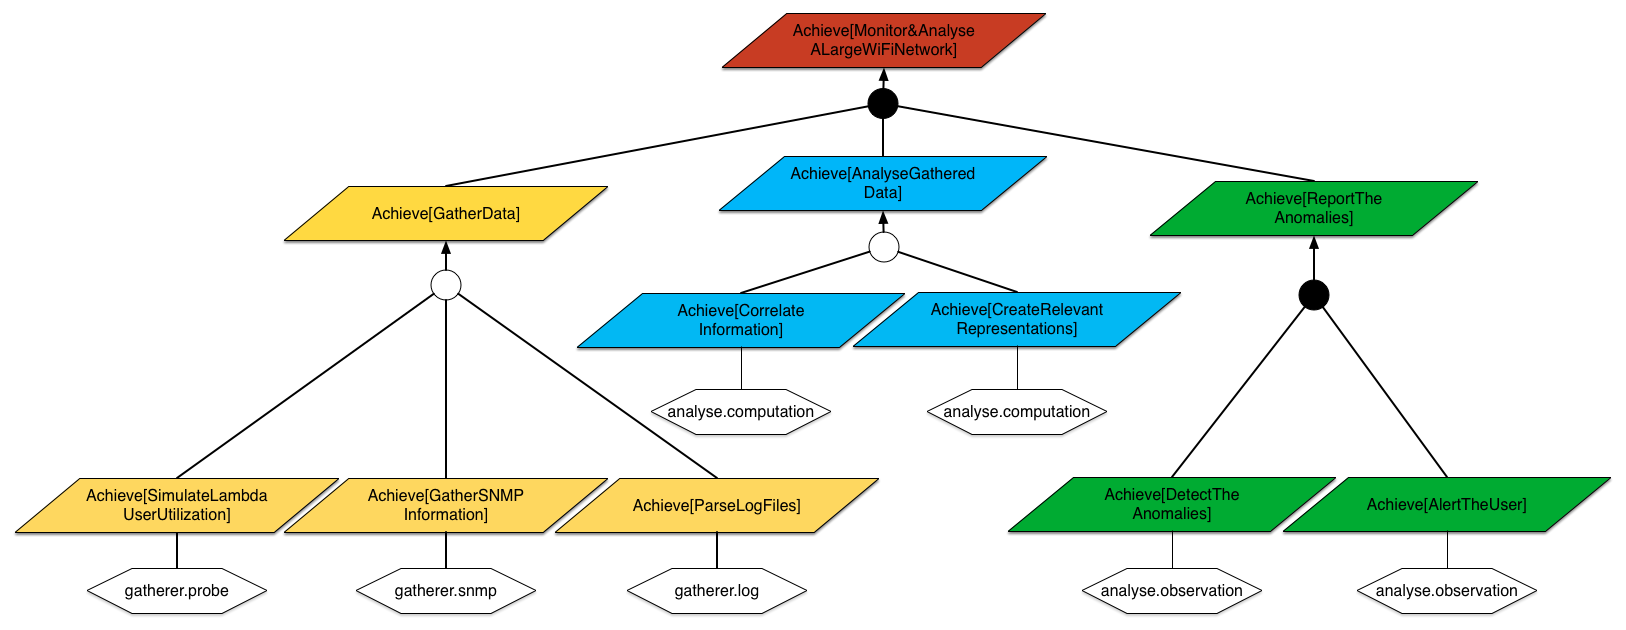
\includegraphics[width=1.1\linewidth]{Pictures/chapter3/goals2.png}
	\caption{Pseudo Goal Model}
\end{figure}

All these requirements come from the meetings we had with the SGSI during the implementation of this monitoring tool. We discussed about what sources of data we could use for this system and what are the information we could deduct from those data and from the analysis the tool performs on them. It is quite important to determine what are the goals and how we will achieve them. This rather simple model allows us to focus on one task at a time without loosing the final purpose of this project.

\subsection{Goals Definition}
\begin{description}
  \item[Name] Monitor\&AnalyseALargeWifiNetwork
  \item[Description] The root goal of our system is to allow the network's administrators to understand what is currently happening on the WiFi network.
\end{description}

\begin{description}
  \item[Name] GatherData
  \item[Description] To provide an efficient monitoring tool we have to gather and centralize all the available information. 
\end{description}

\begin{description}
  \item[Name] SimulateLambdaUserUtilization
  \item[Description] We need to evaluate how the users are perceiving the performances of the network when they use it.
\end{description}

\begin{description}
  \item[Name] GatherSNMPInformation
  \item[Description] We have to record the states of the Controller and access points through time using the \texttt{SNMP} protocol.
\end{description}

\begin{description}
  \item[Name] ParseLogFiles
  \item[Description] We have to be able to understand the information contained in log files generated by the Controller, \texttt{RADIUS} and \texttt{DHCP} servers.
\end{description}

\begin{description}
  \item[Name] AnalyseGatheredData
  \item[Description] Once data are available, we need to analyse them and make comparison between them.
\end{description}

\begin{description}
  \item[Name] CorrelateInformation
  \item[Description] We put related data together in order to generate new information.
\end{description}

\begin{description}
  \item[Name] CreateRelevantRepresentations
  \item[Description] Our results have to be understood by the users through relevant and dynamic graphical representations.
\end{description}

\begin{description}
  \item[Name] ReportTheAnomalies
  \item[Description] More than analyzing data, the system has to be able to alert the administrators of anomalies.
\end{description}

\begin{description}
  \item[Name] DetectTheAnomalies
  \item[Description] Anomalies have to be defined precisely and the system has to use those rules to record deviant network behaviors.
\end{description}

\begin{description}
  \item[Name] AlertTheUser
  \item[Description] The system communicate and displays the anomalies to the users.
\end{description}


\section{Architecture}
In our system's architecture, we have two very distinct main entities. The first entity, called the \texttt{Gatherer}, is responsible for collecting all the information available on the network. This component has the responsibility to keep the operational database up to date and in a consistent state. The second entity of the application, the \texttt{Analyser}, is handling the analysis process made with all that gathered information. Upon these two key processes, we also add an \texttt{Alert System} that produces warnings whenever network anomalies, such as disconnected access points, are spotted. These three parts have to be as independent as possible but also have to be able to communicate between them efficiently. We have designed them by keeping two rules in mind: \textit{modularity} and \textit{simplicity}. The following subsections give more detailed information about these two main entities.

\begin{figure}[H]
\centering
	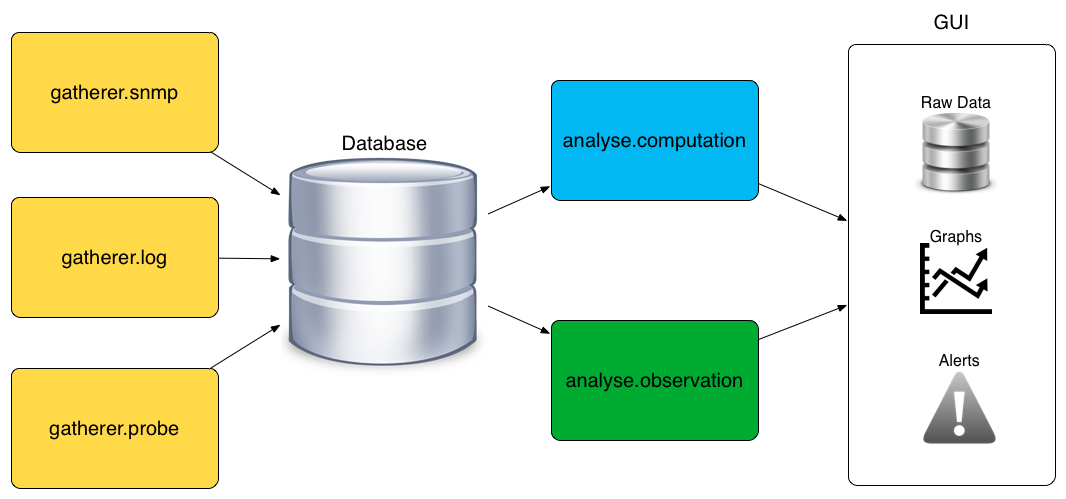
\includegraphics[width=1\linewidth]{Pictures/chapter3/structure.png}
	\caption{Architecture}
\end{figure}


\subsection{Gatherer}
This first main entity of the monitoring application is constituted of several modules that allow it to communicate with the various network data sources. Each module is responsible for collecting a particular kind of information and each one of them has to insert those gathered data into the database. As the information come from heterogeneous sources, before inserting them into the database, each piece of information has to be understood and transformed into coherent entries that can be related to others. Without such transformations, the different possible analysis would be rather limited and not really interesting. The goal we focus on here is \textit{Achieve[GatherData]} and its refinements. Let's now discuss the various sources of information we use in our monitoring tool.

\subsubsection{Log Files}

The first kind of information our monitoring tool gathers are the network component's log files. For each component of the infrastructure there is a different type of log file. As a reminder, these are the three main network components:

\begin{itemize}
  \item \texttt{RADIUS} server
  \item \texttt{DHCP} servers
  \item Controller
\end{itemize}

Each second, these three elements generate several entries in their respective log file and the main difficulty is to make a first sorting among all those data. A part of them is just informational and does not bring any useful information about the state of the network. Such messages will never be used during the analysis process and thus, do not need to be stored in the database. Another part of the log files are just repetition of others. In fact, since each component produces its own logs independently, some of them can overlap and represent the same information. Redundant information are useless and the same piece of information does not need to be stored twice in the database. This might seem to be a negligible issue but in consideration of the quantity of information proceeded by the application, an overloading of the database can cause severe performance issues during the analysis phases. For example, we can see that each time we have two logs \texttt{\%APF-6-RADIUS\_OVERRIDE\_DISABLED}\footnote{This error informs that the attributes sent by the Radius can not override the ones defined for that VLAN}, a third \texttt{\%LOG-6-Q\_IND} appears.\\

\begin{lstlisting}[frame=single,breaklines=true,caption={Example of useless WiSM logs}]
2013-10-21T17:26:00.957695+02:00 192.168.251.178 WiSMPythagore-B: *Dot1x_NW_MsgTask_0: Oct 21 17:26:00.915: %APF-6-RADIUS_OVERRIDE_DISABLED: apf_ms_radius_override.c:204 Radius overrides disabled, ignoring source 2 
2013-10-21T17:26:00.958457+02:00 192.168.251.178 WiSMPythagore-B: *Dot1x_NW_MsgTask_0: Oct 21 17:26:00.916: %APF-6-RADIUS_OVERRIDE_DISABLED: apf_ms_radius_override.c:204 Radius overrides disabled, ignoring source 4 
2013-10-21T17:26:00.985806+02:00 192.168.251.178 WiSMPythagore-B: *Dot1x_NW_MsgTask_0: Oct 21 17:26:00.943: %LOG-6-Q_IND: apf_ms_radius_override.c:204 Radius overrides disabled, ignoring source 4 [...It occurred 2 times.!]
\end{lstlisting}

That's typically the kind of sorting process we perform during the gathering and parsing phases.

The ideal way of gathering these information would be to import them directly from the sources into our server at our convenience. This way, we could manage and optimize the processing of the data. The data would be fetched periodically without overloading the server. But as we will see in the following chapter, we are not able to achieve that. Instead, the log files have to be fetched manually by the users.


\subsubsection{SNMP Queries}

The second kind of gathered data is constituted of \texttt{SNMP} queries. Indeed, the \texttt{SNMP} protocol allows us to retrieve information on the controller in real-time. The module handling the \texttt{SNMP} requests can update the information about the current state of each access point or any client. This brings a lot of interesting data regarding the users of the network but at a cost. The main drawback of using this protocol is that the requests are quite heavy. We cannot make requests every time because it requires a lot of resources from the controller and from our server. In consequence, we have to find the right balance between keeping the database updated and not overloading the controller with \texttt{SNMP} requests. 

The most important information that we extract are the status of every access point on the network. We are also able to see which access points are actually associated with the controller. A lot of statistics, such as the load of the AP, are also available. The same holds for the clients associated to an access point. Each mobile station is indexed by the controller and statistics about it are recorded.


\subsubsection{Active Monitoring}
Finally, we have also implemented an active monitoring and data gathering process in the form of a \texttt{C} program running on \texttt{OpenWrt} Linux \cite{openwrt} routers. The purpose of this element is to simulate a typical user behaviour that connects to the UCL's WiFi network in order to collect data about the overall network performance perceived by that user. Indeed, we cannot be aware of what the user is actually experiencing on the network by only looking at \texttt{SNMP} requests or log files. For this active part, we use an unmodified version of \texttt{wpa\_supplicant} in combination with our \texttt{C} program. We run a connection loop in which the supplicant tries to connect to each of the five WiFi networks available on the Louvain-la-Neuve's campus and we monitor what happens during these connection establishments. We record the time duration of each step and observe which access points are chosen for each network and what is the environment of the router. Plus we also perform some availability and reachability tests on a collection of services and websites we have selected. The purpose is to mimic a client surfing the Internet by using the wireless connection previously established. Using those information we can give an estimation of the overall quality of the network.


\subsection{Analyser}
The \emph{gatherer} only collects and puts available information together. It does not bring anything new. The analyse component will use that data and the links between them to intelligently extract useful information about the network state. For example, the \texttt{SNMP} protocol shows the number of people associated with a given access point but only an analysis through a period time allows us to detect, and even forecast, overload in the network. This component manages all the analysis processes on the database and the storage of the results over time.


\subsection{Database}
The database has to be able to represent each kind of information and manage all the links between them. It is not hard to create entries for a log file but the difficulties appear when we make links with other entities and have to keep them in a coherent state. Several questions raised when we tried to design our database. For example, if a client is no more associated with an access point do we have to remove it from the database or not. Such questions can seem futile but may have deep implications on the database performances. 

Our choice is to clearly separate the different domains of data. Trying to make a link between each element could create inconsistencies and make the analysis harder. That is why each category of information has its own tables and links are only made when they are clearly present in the source data. This does not mean that we don't cross the information, it simply means that we let the data independent and we link them only when we need to perform an analysis. As there are plenty of ways to organize them, we preferred to keep them neat and avoid to mix them in the gathering part.

The following figure details the architecture of our database.
\begin{figure}[H]
\centering
  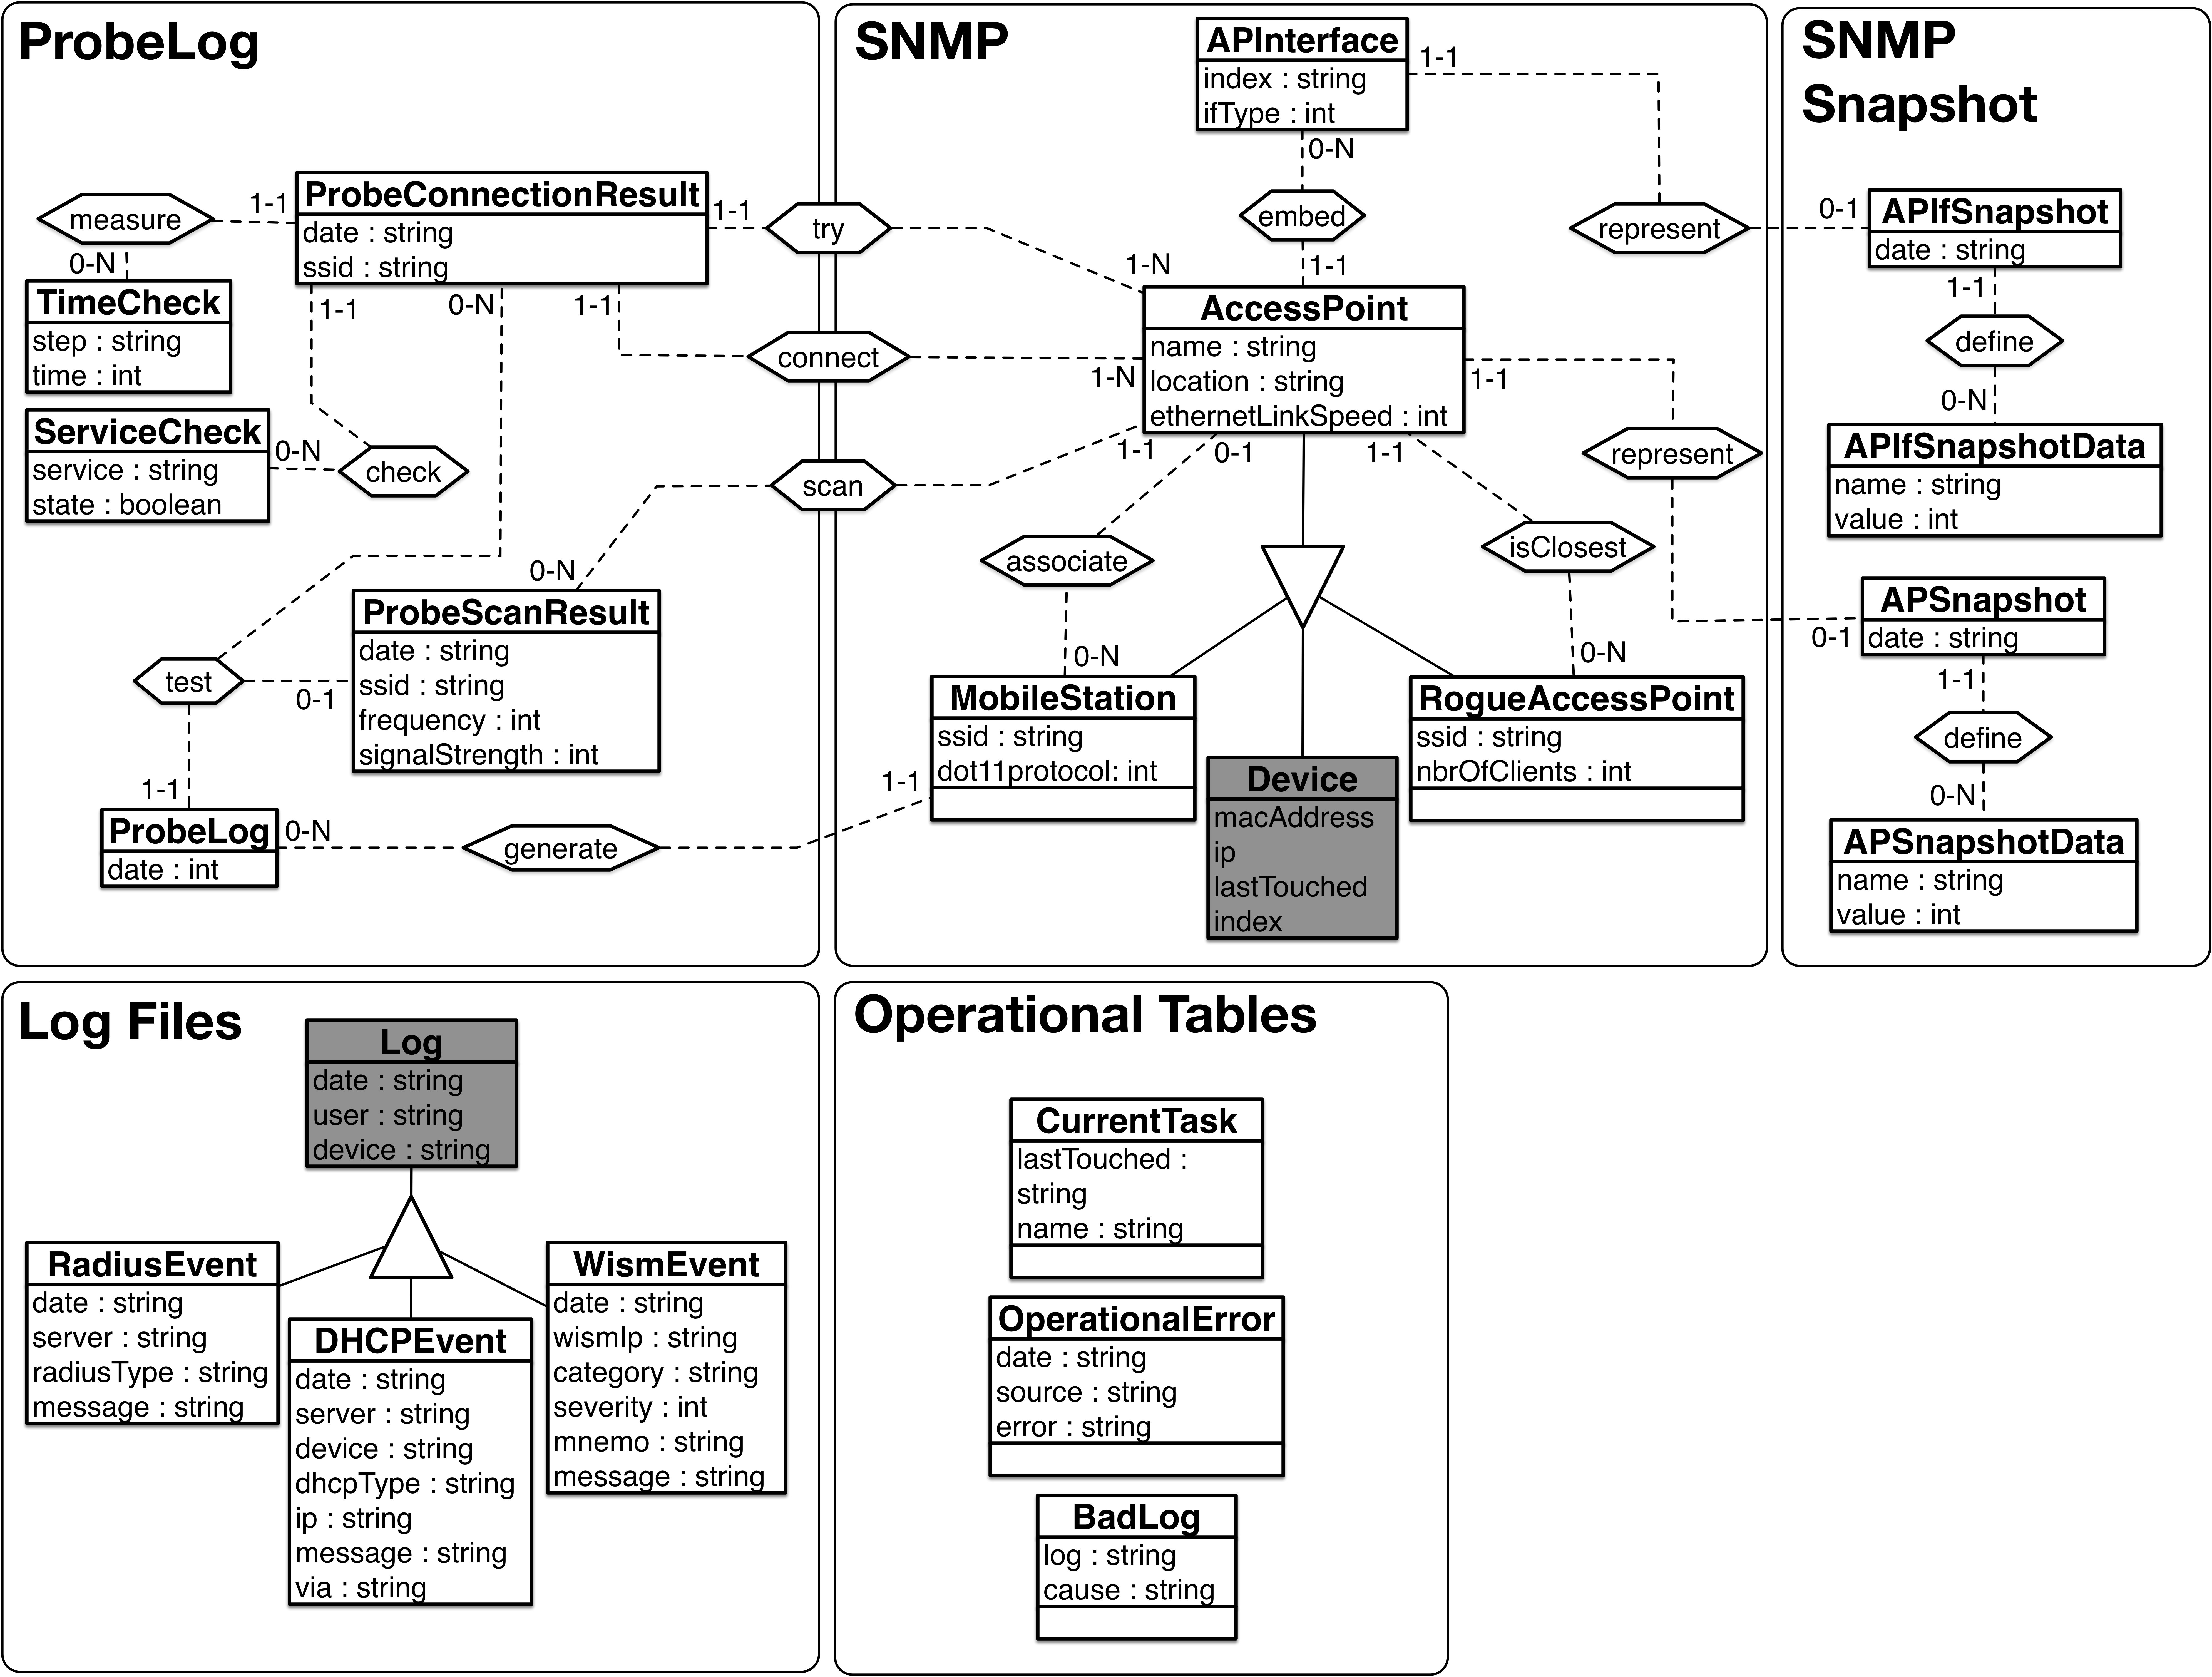
\includegraphics[width=1\linewidth]{Pictures/chapter3/db2.png}
  \caption{Interconnections with the UCL's network infrastructure}
\end{figure}


\section{Link with the Infrastructure}
Our monitoring tool needs to be directly plugged into the network infrastructure in order to be efficient and to display interesting results. For each data source, we have to define a point of communication in our system between the source and one of our modules. The data is not centralized and we have to manage how we access it and try to define a right balance between performances and respect of the external components which host the network information. For example, we can't overload \texttt{SNMP} agents with requests.

The following figure represents the interconnections the UCL's network have with our monitoring system.

\begin{figure}[H]
\centering
	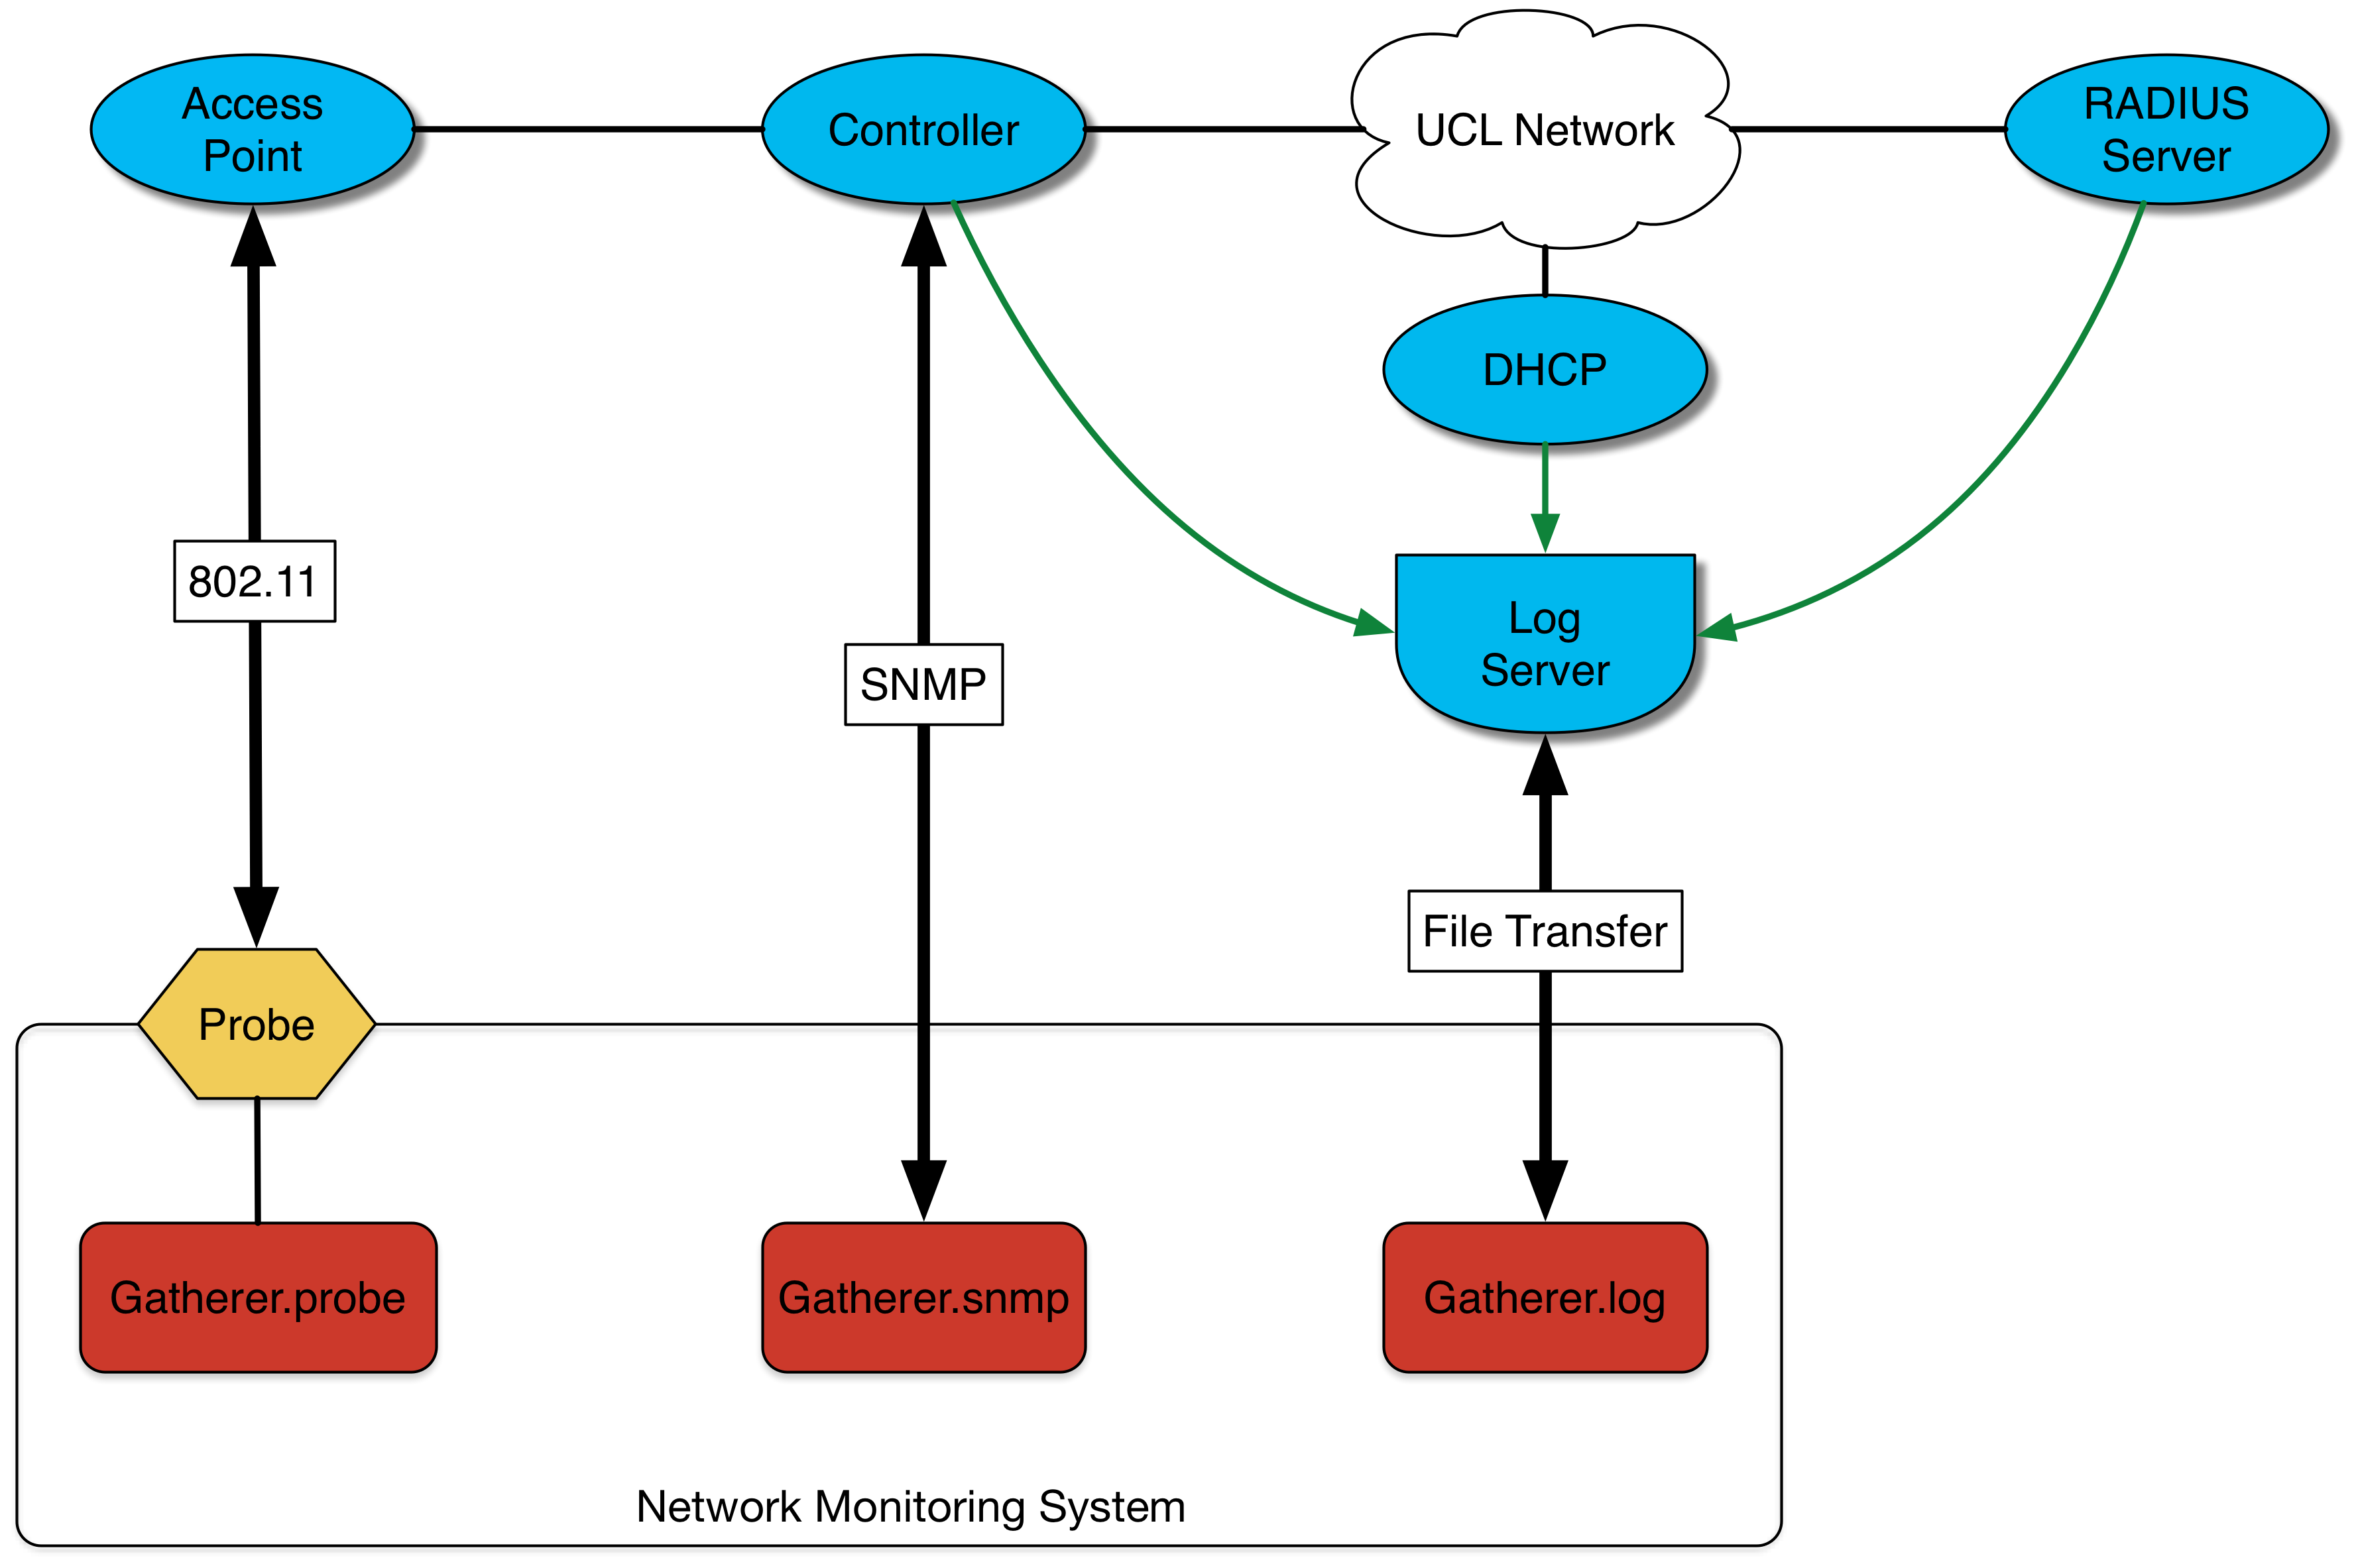
\includegraphics[width=.8\linewidth]{Pictures/chapter3/interactions.png}
	\caption{Interconnections with the UCL's network infrastructure}
\end{figure}


\subsection{Controller}
The controller hosts all the \texttt{SNMP} data about itself or the access points. Our system collects them directly on the controller periodically. As shown in the figure above, it is the \texttt{Gatherer.snmp} that handles all the transactions. As said before, there are two controllers hidden behind one virtual IP. That configuration permits to always perform the request to the same address and only the active controller will answer.

\subsection{Access Points}
The \texttt{OpenWrt}  probes associate with an access point and the resulting messages are sent to the server. There is no special configuration required as the devices need to operate as a lambda user. The initial configuration of the devices, such as the wireless driver, stays unmodified.

\subsection{Log Server} 
The log files are stored on a dedicated server and the administrator retrieves manually them from there by file transfer. In an ideal situation, we would automatize the gathering of those files and process them periodically too.

\section{Summary}
This chapter presented the architecture of the monitoring tool and how the components work together in order to meet the requirements and the goals defined in the first step. The system is divided into two distinct parts, the data gatherer and the information analyser, in order to get modularity and simplicity. The next chapter covers the implementation design and the deployment of the modules contained in those two distinct parts.




